Along with understanding what drives memorability of objects in a scene, our work also makes available the very first dataset containing the ground truth memorability of constituent objects from a highly diverse image set. In this section, we show that our dataset can be used to benchmark computational models and serve as a stepping stone in the direction of object memorability prediction.

\noindent
\textbf{Baseline models:} As a first step, we propose a simple
baseline model that utilizes a conv-net \cite{krizhevsky12},
\cite{jia14} trained on the ImageNet database \cite{deng09}. Since
object categories play an important role in determining object
memorability (Section \ref{sec:obLabel}), and deep learning models have
recently been shown to achieve state-of-the-art results in various
recognition tasks, including object recognition and object
categorization \cite{cnn14}, \cite{lee2009convolutional}, we believe
that this simple model can serve as a good initial baseline for object
memorability prediction. We first generated object segments by using
MCG, a generic object proposal method proposed in
\cite{arbelaez14}. Next, we trained an SVR using $6$-fold
cross-validation on the original segments to map deep features to
memorability scores. We then used this model to predict the
memorability scores for the top K ($K=20$) segments (obtained via the
ranking scores provided by the MCG algorithm) for each image. After
obtaining the predicted memorability scores, the memorability maps
were generated by averaging the top $K$ segments at the pixel
level. 
Since image features like SIFT \cite{lowe04} and HOG
\cite{dalal05} have previously been shown to achieve good performance
in predicting image memorability \cite{isola11}, \cite{isola14}, we
built a second baseline model using these features for
comparison. Training and testing of this model was performed similar
to the deep-net baseline model. 

\noindent \textbf{Evaluation: } To evaluate the accuracy of the predicted memorability maps, we computed the rank correlation between the mean predicted memorability score inside each of the original object segments and their ground truth memorability scores. From Figure \ref{fig:benchmark}, we first note that our deep-net baseline model, DL-MCG performs considerably well ($\rho = 0.39$). In contrast, the baseline model trained using HOG and SIFT features, H+S exhibits much lower overall performance ($\rho = 0.27$). Saliency maps generated from saliency algorithms are also likely to have some degree of overlap with memorability and are therefore worth comparing to our baseline, especially given the absence of alternative memorability prediction methods\footnote{The only other algorithm that generates memorability maps was proposed in \cite{khosla12}. We contacted the authors and they said they will be releasing an updated version of their paper and codes soon. We will add it to the comparison once they release the code.}. Thus, we also included $8$ state-of-the-art-saliency methods GB \cite{gb}, AIM \cite{aim}, DV \cite{dv}, IT \cite{it}, GC \cite{gc}, PC \cite{pc}, SF \cite{sf}, and FT \cite{ft} to our comparison (some of the top performing methods according to benchmarks in \cite{borji13}, \cite{borji12}).  Results from figure \ref{fig:benchmark}) show that the H+S baseline is outperformed by most saliency methods. Thus, even though models using SIFT and HOG have previously demonstrated high predictive power for image memorability, they may not be as well suited for the task of predicting object memorability. The deep-net baseline model, DL-MCG performs better than all other saliency methods and only PC ($\rho=0.38$), SF ($\rho=0.37$), and GB ($\rho=0.36$) show performance comparable to the model. A common factor between these saliency methods is that they explicitly add center bias to their implementation. Even though memorability exhibits lesser center bias when compared to eye fixations, it still tends to biased slightly towards the center due to photographer bias (Section \ref{sec:fix}), which could be a  part of the reason for the high performance of these methods. Despite this, DL-MCG performs favorably against them and is potentially much better suited for memorability prediction on a wide range of datasets. Thus, we recommend in the future, memorability algorithms compare their methods against our DL-MCG baseline. While DL-MCG performed fairly well, part of the performance of this model is dependent on the quality of the segmentations used. For this reason, we also consider the upper bound of our current predictive power by showing the results for our model containing predictions on the original segments (referred to as DL-UL in Figure \ref{fig:benchmark}). Interestingly, the accuracy of this model is very high and close to human performance ($\rho = 0.7$). This demonstrates that the deep-net model has high predictive ability that is suppressed most heavily by constraints of the segmentation task. The main insight of our evaluation is that deep features serve as strong predictors of memorability and selection of higher quality segments can potentially lead to improved memorability prediction algorithms.

\begin{figure}[t]
\centering
\subfigure{\centering 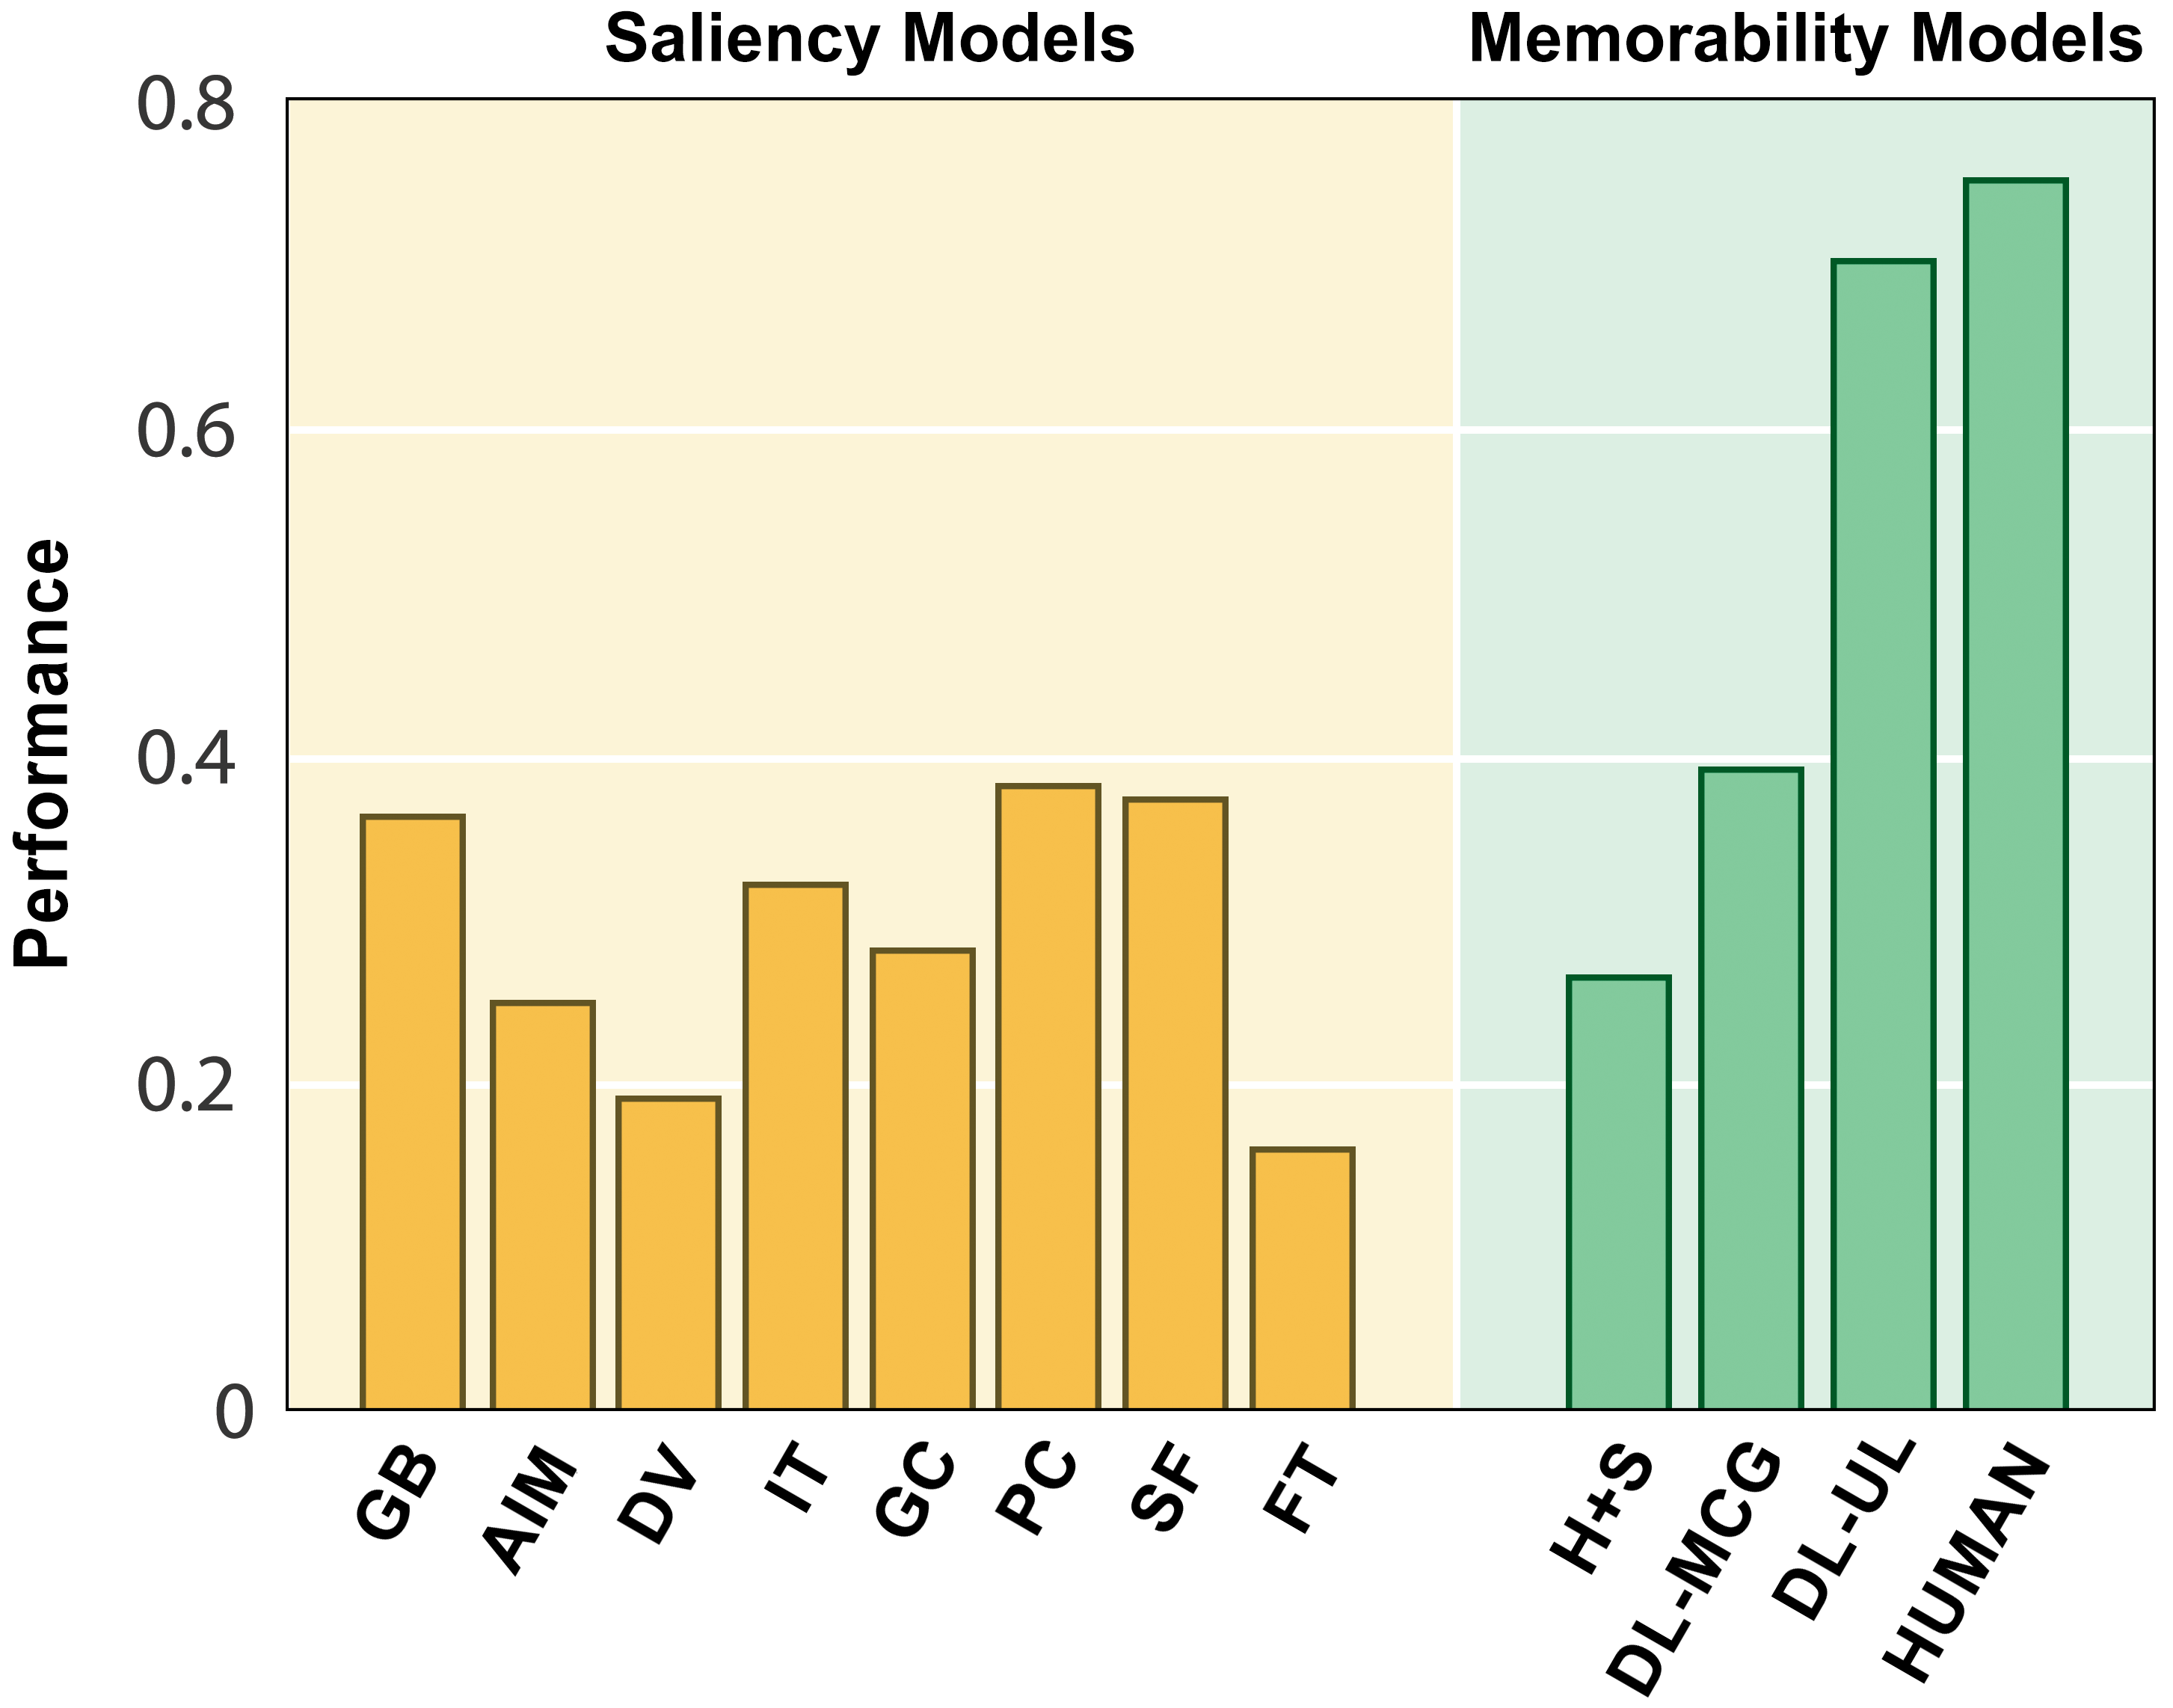
\includegraphics[width=0.5\textwidth]{figures/results/benchmark/comparison.png}}
\vspace{-5mm}\caption{\footnotesize\textbf{Main task.} add-in later. }\label{fig:benchmark}
\end{figure} 